%\vspace{-0.1in}
\secspace
\section{Introduction}
\secspace
\label{sec:intro}

In this rather atypical hotnets submission we discuss a problem that is quite
(c)old, albeit one that has re-emerged in a new context, and admit that we have
no idea how to solve it completely. Our hope is to draw the community's
attention to this problem, and re-ignite research in this area.

The problem is deadlock formation in lossless networks.

Driven by the need for ultra-low latency, high throughput and low CPU overhead,
major cloud service providers are deploying Remote Direct Memory Access (RDMA) in
their datacenter networks~\cite{dcqcn,timely}. Among the
available RDMA technologies,  RDMA over Converged Ethernet (RoCE)~\cite{roce} is
a promising one as it is compatible with current IP and Ethernet based
datacenter networks.

The deployment of RoCE requires Priority-based Flow Control (PFC)~\cite{pfc} to
provide a lossless L2 network. With PFC, packet loss can be avoided by letting a
switch pause its immediate upstream device before buffer overflow occurs.
However, PFC can cause deadlock problem. Deadlock refers to a
standstill situation: there is a cyclic buffer dependency among a set of
switches. Any switch in the cycle holds all the buffer needed by its upstream
switch, and meanwhile is waiting for its downstream switch to release some
buffer and resume its packet transmission. A simple scenario is illustrated in
Figure~\ref{fig:deadlock_example}.

It is easy to see that when deadlock occurs, no switch in the cycle can proceed.
Further, throughput of the whole network or part of the network will go to zero
due to the backpressure effect of PFC pause. 

It is often believed that such deadlocks cannot occur in
clos-structured datacenter networks, since a loop cannot form in such networks
with valley-free routing~\cite{dcqcn}.  However~\cite{rdmascale} has shown that
deadlocks can indeed occur in such network, typically as a result of
misconfiguration. We now believe that deadlocks can also occur when transient
loops form in clos structured networks. In our datacenters, these can happen as
BGP\footnote{In our datacenters, we use BGP for routing, with each switch being
a private AS.} re-routes around link failures. In SDN-based datacenters,
transient loops can occur
during updates~\cite{dionysus}.

Hence some mechanism for handling the deadlock problem must be used when
deploying RDMA in datacenter networks.  These mechanisms fall in two broad
categories. {\em Reactive} mechanisms/systems detect that a deadlock has formed,
and then try to break it by resetting links/ports/hosts etc.  These mechanisms
are inelegant, disruptive, and should be used only as a last resort.  We do not
consider them further in this paper.  {\em Proactive} deadlock prevention is a
more principled approach to this problem.  Prior work on deadlock prevention can
be classified into two categories including 1) \textit{Routing restriction-based
approach}~\cite{tcpbolt,flich2012survey}. The idea of this approach is to ensure
that no cyclic buffer dependency exists in the network by limiting the routing
paths used in each priority class;  2) \textit{buffer management (structured
buffer pool) based approach}~\cite{gerla1980flow,karol2003prevention}. This
approach divides switch buffer into several buffer classes. A packet is allowed
to access more buffer classes as it travels greater distance in the network. It
can be proved that as long as the number of buffer classes is no smaller than
the hop count of the longest routing path, there will be no cyclic buffer
dependency.

\begin{figure}
\centering
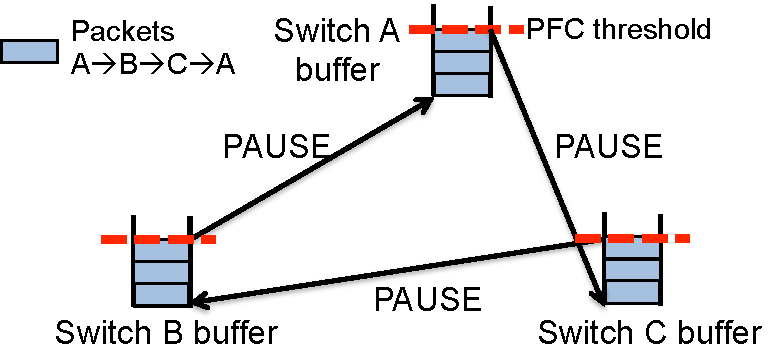
\includegraphics[width=0.25\textwidth] {figs/deadlock}
\vspace{-0.15in}
\caption{PFC-induced deadlock: simple illustration}
\vspace{-0.25in}
\label{fig:deadlock_example}
\end{figure}

Both these approaches to deadlock prevention have some important drawbacks.
Approaches based on routing restriction usually waste link bandwidth and limit
throughput performance, while buffer management based approach introduces
non-trivial deployment complexity. These drawbacks can be viewed as the cost of
eliminating cyclic buffer dependency in the network. While avoiding cycle buffer
dependency gurantees a deadlock-free network, it may not be always feasible to
pay these costs.

Thus, we take step back and ask: Is cyclic buffer dependency a
necessary condition for deadlock formation, or is it a sufficient condition? If
it is only a {\em necessary} condition, can we focus on {\em sufficient}
conditions, and guarantee deadlock freedom, without  eliminating cyclic buffer
dependency?

To answer the above questions, we studied several representative deadlock cases.
First, we find that cyclic buffer dependency is
just a necessary condition for deadlock. In some sense, this is trivially true:
if no flow is sending any data, there will obviously be no deadlock, regardless
of cyclic buffer dependency.  However, there are also several non-trivial cases
where cyclic buffer dependency is met, all flows are active, but there is no
deadlock.  Second, we find that even if all the links in a switch cycle are
paused simultaneously, deadlock may still not occur.  These findings
indicate that prior solutions are {\em too} conservative. 

So, in this paper, we shall try to understand the {\em sufficient} conditions
for deadlock formation, which we conjecture to be far easier to ameliorate than
the {\em necessary} conditions. As mentioned earlier, we do not yet have a
precise characterization of the sufficient conditions. Yet, we have made some
headway, which allows us to sketch a few possible solutions to the problem.

